%%%%%%%%%%%%%%%%%%%%%%%%%%%%%%%%%%%%%%%%%%%%%%%%%%%%%%%%%%%%%%%%%%%%%%%%%%%%%%%%%
%																				%
%	TRABAJO:	Trabajo Final													%
%				Especialidad en Ingenier�a en Sistemas de Informaci�n			%
%																				%
%		Titulo:	Procesamiento de Datos en Tiempo Real							%
%																				%
%		Autor:	Juli�n Nonino													%
%																				%
%	DOCUMENTO PRINCIPAL															%	
%																				%
%	A�o: 2016																	%
%																				%
%%%%%%%%%%%%%%%%%%%%%%%%%%%%%%%%%%%%%%%%%%%%%%%%%%%%%%%%%%%%%%%%%%%%%%%%%%%%%%%%%

\documentclass[a4paper,12pt,openright,twoside]{book}

% Paquetes
	% Idioma y codificacion de caracteres
		\usepackage[spanish]{babel}		
		\usepackage[latin1]{inputenc}
		\usepackage{csquotes}
	% Figuras
		\usepackage{graphicx}
		\usepackage{subfigure}
		\usepackage{float} % Para posicionar im�genes donde uno quiera. Solo hay que poner la opcion [H]
	% Apendice
		\usepackage{appendix}
	% Margenes
		\usepackage{anysize}
	% Tabla de conteido
		\usepackage[tight]{shorttoc}
	% Matematica
		\usepackage[cmex10]{amsmath}
		\usepackage{amssymb}
	% Colores
		\usepackage{color}
		% Definicion de colores
			\definecolor{dkgreen}{rgb}{0,0.6,0}
			\definecolor{gray}{rgb}{0.5,0.5,0.5}
			\definecolor{mauve}{rgb}{0.58,0,0.82}
			\definecolor{violeta}{RGB}{127,0,85}
	% Insertar c�digo
		\usepackage{listings}
		\lstdefinestyle{bash}{
   			language=Bash,
   			showspaces=false,
   			showstringspaces=false,
   			basicstyle=\ttfamily,
   			columns=flexible,
   			stringstyle=\color{javastring},
   			keywordstyle=\color{violeta}\ttfamily\textbf,
   			commentstyle=\color{dkgreen}\ttfamily\textit
 		}
	% URLs
		\usepackage{url}
	% Referencias
		\usepackage{hyperref}
		\usepackage[style=numeric,backend=bibtex,sorting=none]{biblatex}
		\addbibresource{./informe/referencias.bib}

% Margenes
	% Controla los m�rgenes {izquierda}{derecha}{arriba}{abajo}
		\marginsize{3cm}{3cm}{2.5cm}{2.5cm}

% Encabezados
	\pagestyle{headings}
		
% Documento
\begin{document}
 
	% Reeescritura de comandos
		\renewcommand{\lstlistingname}{C�digo}
		\renewcommand{\appendixname}{Ap�ndice}
		\renewcommand{\appendixtocname}{Ap�ndice}
		\renewcommand{\tablename}{\textbf{Tabla}} 	% Para poner la palabra en mayusucula
		\renewcommand{\figurename}{\textbf{Figura}} % Para poner la palabra en mayuscula
		\renewcommand{\contentsname}{�ndice}
		\renewcommand{\listtablename}{�ndice de tablas}
		\renewcommand{\listfigurename}{�ndice de Figuras}

		\setcounter{secnumdepth}{3} % Para numerar subsubsecciones
		\setcounter{tocdepth}{3}	% Para incluir subsubsecciones en la TOC	
	
	% INICIO DE LA PRIMERA PARTE. Resumen ejecutivo
 		\frontmatter
 		% Portada
 			\begin{titlepage}
 				%%%%%%%%%%%%%%%%%%%%%%%%%%%%%%%%%%%%%%%%%%%%%%%%%%%%%%%%%%%%%%%%%%%%%%%%%%%%%%%%%
%																				%
%	TRABAJO:	Trabajo Final													%
%				Especialidad en Ingenier�a en Sistemas de Informaci�n			%
%																				%
%		Titulo:																	%
%																				%
%		Autores:	Julian Nonino												%
%																				%
%	Portada																		%	
%																				%
%	A�o: 2016																	%
%																				%
%%%%%%%%%%%%%%%%%%%%%%%%%%%%%%%%%%%%%%%%%%%%%%%%%%%%%%%%%%%%%%%%%%%%%%%%%%%%%%%%%

% PAGINA ANTERIOR
	\vspace*{0.15in}

	\begin{center}		
	
		\begin{LARGE}
			\textbf{Procesamiento de Datos en Tiempo Real}
		\end{LARGE}
		\\
		\vspace*{0.15cm}
		\begin{Large}
			\textbf{Conceptos y An�lisis de Herramientas}
		\end{Large}
		
		\vspace*{0.15cm}
		\rule{15cm}{0.1mm} 
		\vspace*{0.15cm}
		\begin{Large}Especializaci�n en Ingenier�a en Sistemas de
		Informaci�n\end{Large}\\
	
		\vspace*{2cm}
	
		\begin{Huge}
			Juli�n Nonino
		\end{Huge}
		\\
		
		\vspace*{2cm}
		
%		\begin{Large}
%			Director
%			\\
%			\vspace*{0.5cm}
%			Mart�n Miceli
%		\end{Large}
		
		\vspace*{4.5cm}
		
		\begin{figure}[H]
			\centering
			
\includegraphics[width=.10\linewidth]{./portada/logo_utn}
		\end{figure}	
		
		
		\begin{large}Universidad Tecnol�gica Nacional\end{large}\\
		\vspace*{0.25cm}
		\begin{large}Facultad Regional C�rdoba\end{large}\\
		\vspace*{0.25cm}
		\begin{large}Direcci�n de Posgrado\end{large}\\
		\vspace*{0.5cm}
		C�rdoba\\
		- 2016 -
	\end{center}

% PAGINA POSTERIOR
	\newpage
	\mbox{}
	\thispagestyle{empty}
	
 				\thispagestyle{empty}
 			\end{titlepage}
 		% Resumen
 			% Resumen ejecutivo
 				%%%%%%%%%%%%%%%%%%%%%%%%%%%%%%%%%%%%%%%%%%%%%%%%%%%%%%%%%%%%%%%%%%%%%%%%%%%%%%%%%
%																				%
%	TRABAJO:	Trabajo Final													%
%				Especialidad en Ingenier�a en Sistemas de Informaci�n			%
%																				%
%		Titulo:	Procesamiento de Datos en Tiempo Real							%
%																				%
%		Autor:	Juli�n Nonino													%
%																				%
%	Resumen Ejecutivo															%	
%																				%
%	A�o: 2016																	%
%																				%
%%%%%%%%%%%%%%%%%%%%%%%%%%%%%%%%%%%%%%%%%%%%%%%%%%%%%%%%%%%%%%%%%%%%%%%%%%%%%%%%%

\chapter*{Resumen Ejecutivo}

En los �ltimos a�os, con las llegada de las Redes Sociales, Big Data, Internet
de las Cosas, entre otras, la cantidad de datos generados creci�
exponencialmente. Paralelamente, se vi� incrementada la necesidad de tomar
acciones en base a dichos datos en el menor tiempo posible. En medio de �ste
fen�meno, surgen los sistemas en la nube, con escalabilidad para crecer y
decrecer en base a los requerimientos de procesamiento de cada momento. En ese
marco surgen nuevas tecnolog�as como \emph{Docker}, \emph{Apache Zookeeper},
\emph{Apache kafka} y \emph{Apache Storm}.

Con \emph{Docker} es posible utilizar contenedores de software independientes
que pueden comunicarse con otros contenedores proporcionando una capa de
virtualizaci�n sencilla a nivel de sistema operativo Linux. Su principal
ventaja radica en la facilidad de despligue de apliacaci�n que provee su uso.

\emph{Apache Zookeeper} surge como un servicio de coordinaci�n de alto
rendimiento para aplicaciones distribuidas. Expone servicios comunes, tales como
nomenclatura, manejo de las configuraciones, sincronizaci�n, etc�tera. Entre
otras funciones, se utiliza para implementar consenso, manejar grupos, elecci�n
de nodo l�der y protocolos de presencia.

\emph{Apache Kafka} es un sistema de mensajes distrubuido, particionado y con
replicaci�n. Su principal objetivo es recibir datos desde el mundo exterior al
sistema y garantizar su diponibildiad para otros componentes del sistema que
necesiten leerlos y procesarlos.

\emph{Apache Storm} es una herramienta de procesamiento de datos en tiempo real
de c�digo abierto y gratuita creada por Twitter y luego liberada bajo la �rbita
de los proyectos Apache. La finalidad de Storm es proveer un mecanismo confiable
para procesamiento de flujos de datos ilimitados. De acuerdo a su documentaci�n,
Storm es capaz de procesar un mill�n de tuplas de datos por segundo por nodo.
Provee caracter�sticas de escalabilidad, tolerancia a fallos, garant�as de que
todos los datos ser�n procesados, etc�tera\cite{ApacheStorm097}.

Utilizando dichas tecnolog�as se generan im�genes de Docker para la conformaci�n
de un cl�ster de Apache Zookeeper, uno de Apache Kafka y otro de Apache Storm.
Se utilizar� Docker Compose para levantar los servicios necesarios. Para el
alcance de �sta prueba de concepto, todos los servicios correr�n en el mismo
servidor pero, para aprovechar las propuesta de alta disponibilidad y
escalabilidad que ofrecen �stas tecnolog�as, ser�a recomedable que cada nodo de
cada uno de los servicios corra en un servidor independiente.

Se desarrolla una aplicaci�n Java para enviar datos a Apache Kafka en el sistema
y una topolog�a de Apache Storm que buscar� los datos en el servicio de Apache
Kafka y los dejar� listos para ser procesados.

Se mostrar� como se realiza el despliegue del sistema con tres nodos de
\emph{Apache Zookeeper}, tres nodos de \emph{Apache Kafka} y tres nodos para
\emph{Apache Storm}, uno para el nodo \emph{Nimbus}, otro para el nodo
\emph{Supervisor} y un nodo para \emph{Interfaz Gr�fica}.

Tambi�n se muestra como se carga la topolog�a desarrollada en el cl�ster de
Apache Storm y luego, como enviarle datos al sistema mediando una aplicaci�n
Java que act�a como productor de datos para Apache Kafka.

Finalmente, se comprueba que el sistema, est� recibiendo datos (Apache Kafka) y
efectivamente, llegan al sistema de procesamiento (Apache Storm).

La prueba de concepto puede ser extendida implementado nuevas topolog�as de
Apache Storm para realizar procesamientos m�s complejos de los datos, utilizar
un servicio en la nube para alojar los servidores. Por otro lado, implementar
mecanismos de auto escalabilidad de cada uno de los servicios para que el
sistema crezca y decrezca dependiendo de las necesidades de procesamiento del
momento. Tambi�n, es posible implementar mecanismos de auto descubrimiento de
servicios para garantizar que al crear o borrar un nodo de alg�n servicio el
sistema continue funcionando de manera �ptima.

 		% Tabla de contenido inicial
 			\shorttableofcontents{Tabla de contenido}{0}
 		
 	%INICIO DEL TEXTO PRINCIPAL
 		\mainmatter
 		% Introducci�n
 			\part{Introducci�n}
 				% Introducci�n
					%%%%%%%%%%%%%%%%%%%%%%%%%%%%%%%%%%%%%%%%%%%%%%%%%%%%%%%%%%%%%%%%%%%%%%%%%%%%%%%%%
%																				%
%	TRABAJO:	Trabajo Final													%
%				Especialidad en Ingenier�a en Sistemas de Informaci�n			%
%																				%
%		Titulo:																	%
%																				%
%		Autor:	Juli�n Nonino													%
%																				%
%	Introducci�n																%	
%																				%
%	A�o: 2016																	%
%																				%
%%%%%%%%%%%%%%%%%%%%%%%%%%%%%%%%%%%%%%%%%%%%%%%%%%%%%%%%%%%%%%%%%%%%%%%%%%%%%%%%%

\chapter{Introducci�n}
	

	
\section{Objetivos}

	El objetivo principal de �ste trabajo es implementar un sistema de procesamiento
	de datos en tiempo real como prueba de concepto utilizando las �ltimas
	tecnolog�as de la industria como son Docker, Apache Zookeeper, Apache Kafka y
	Apache Storm.
	
	\subsection{Objetivos Secundarios}
	
		\begin{itemize}
		    \item Plantear un modelo de generaci�n y procesamiento de datos sencillo que
		    ayude a visualizar el funcionamiento del sistema.
		    \item Demostrar el rol de Apache Zookeeper dentro de los sistemas
		    distribuidos. Mostrar su implementaci�n a trav�s de una prueba de concepto.
		    \item Demostrar el rol de Apache Kafka y Apache Storm dentro de los sistemas
		    de procesamiento de datos en tiempo real.
		    \item Estudiar y utilizar Docker como herramienta de despliegue de los
		    componentes del sistema ayudando a la escalabilidad del sistema.
		    \item Utilizar Docker Compose como mecanismo de despliegue del
		    sistema y conexi�n de los componentes del mismo.
		\end{itemize}

				% Marco Te�rico
					%%%%%%%%%%%%%%%%%%%%%%%%%%%%%%%%%%%%%%%%%%%%%%%%%%%%%%%%%%%%%%%%%%%%%%%%%%%%%%%%%
%																				%
%	TRABAJO:	Trabajo Final													%
%				Especialidad en Ingenier�a en Sistemas de Informaci�n			%
%																				%
%		Titulo:	Procesamiento de Datos en Tiempo Real							%
%																				%
%		Autor:	Juli�n Nonino													%
%																				%
%	Marco Te�rico																%	
%																				%
%	A�o: 2016																	%
%																				%
%%%%%%%%%%%%%%%%%%%%%%%%%%%%%%%%%%%%%%%%%%%%%%%%%%%%%%%%%%%%%%%%%%%%%%%%%%%%%%%%%

\chapter{Marco Te�rico}
\label{chapter_marco_teorico}

\section{Procesamiento de Datos en Tiempo Real}
\label{section_real_time}

	En los �ltimos tiempos, la demanda de procesamiento de flujos continuos de datos
	(data streams) se ha incrementado considerablemente. Esto se debe a que ya no es
	suficiente con procesar grandes vol�menes de datos, adem�s, deben ser procesados
	r�pidamente permitiendo a los sistemas reaccionar ante los eventos lo antes
	posible. Ejemplos de sistemas que necesitan �ste nivel de procesamiento son los
	sistemas de detecci�n de fraude, monitoreo de recursos, comercio, etc�tera.

	\subsection{Big Data}
	
		El t�rmino Big Data, muy utilizado en la actualidad, hace referencia a lo que se
		conoce como las \textbf{\emph{Tres V}}, \emph{Volumen}, \emph{Variedad} y
		\emph{Velocidad}.
		Con ello, se quiere indicar que un sistema Big Data no solo implica trabajar con
		grandes vol�menes de datos, sino que estos datos pueden ser muy variados y se
		deben procesar r�pidamente \cite{Wahner2014}.
	
		\begin{figure}[H]
			\centering
			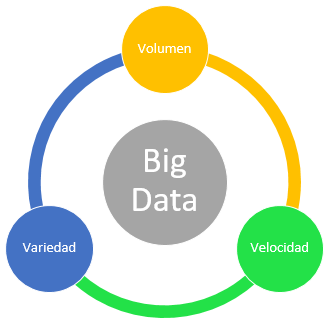
\includegraphics[width=.5\linewidth]{./informe/introduccion/img/real_time/big_data_tres_v}
		\end{figure}

	\subsection{Procesamiento de Flujos de Datos (Stream Processing)}
		
		En contraste a los modelos de procesamiento de datos tradicionales en los cuales
		los datos son primero almacenados, cuando se trabaja un flujo de datos, los
		datos son procesados y analizados mientras entran en el sistema. Esto se
		conoce como procesar datos en movimiento, conectando los procesadores de datos
		con las fuentes que los producen.
					
		Una soluci�n de procesamiento de datos en tiempo real debe ser capaz de:
		\begin{itemize}
		    \item Procesar cantidades enormes de datos permitiendo filtrado, agregaci�n,
		    predicci�n, alertas, reglas, etc�tera.
			\item Respuesta en tiempo real a los mensajes/eventos recibdos.
			\item Asegurar rendimiento y escalabilidad cuando el volumen de datos crece en
			tama�o y/o complejidad.
			\item Integraci�n f�cil y r�pida con la infraestructura y fuentes de datos
			existentes.
			\item R�pida implementaci�n y puesta en producci�n de nuevos requisitos de
			procesamiento.
		\end{itemize}
		
\section{Docker}
\label{section_docker}

	Docker es un proyecto de c�digo abierto que automatiza el despliegue de
	aplicaciones dentro de contenedores de software, proporcionando una capa
	adicional de abstracci�n y automatizaci�n de virtualizaci�n a nivel de sistema
	operativo en Linux. Docker utiliza caracter�sticas de aislamiento de recursos del
	kernel de Linux, tales como \emph{cgroups} y \emph{espacios de nombres
	(namespaces)} para permitir que \emph{contenedores} independientes se ejecuten
	dentro de una sola instancia de Linux, evitando la sobrecarga de iniciar y
	mantener m�quinas virtuales.\cite{WikipediaDocker}
	
	Docker implementa una API de alto nivel para proporcionar contenedores livianos
	que ejecutan procesos de manera aislada.
	Construido sobre las facilidades proporcionadas por el kernel de Linux (nombradas
	anteriormente), un \emph{contenedor} Docker, a diferencia de una m�quina virtual,
	no requiere incluir un sistema operativo independiente. En su lugar, se basa en
	las funcionalidades del kernel y utiliza el aislamiento de recursos y namespaces
	separados para aislar de vista la aplicaci�n del sistema operativo.\cite{WikipediaDocker}

	El soporte del kernel de Linux para los \emph{espacios de nombres} a�sla de vista
	una aplicaci�n del entorno operativo, incluyendo �rboles de proceso, red, ID de
	usuario y sistemas de archivos montados. A su vez, los \emph{cgroups} del kernel
	proporcionan aislamiento de recursos, incluyendo la CPU, la memoria, el bloque de
	E/S y de la red. Desde la versi�n 0.9, Docker incluye la librer�a
	\emph{libcontainer} como su propia manera de utilizar directamente las
	facilidades de virtualizaci�n que ofrece el kernel de Linux.\cite{WikipediaDocker}

	\begin{figure}[H]
		\centering
		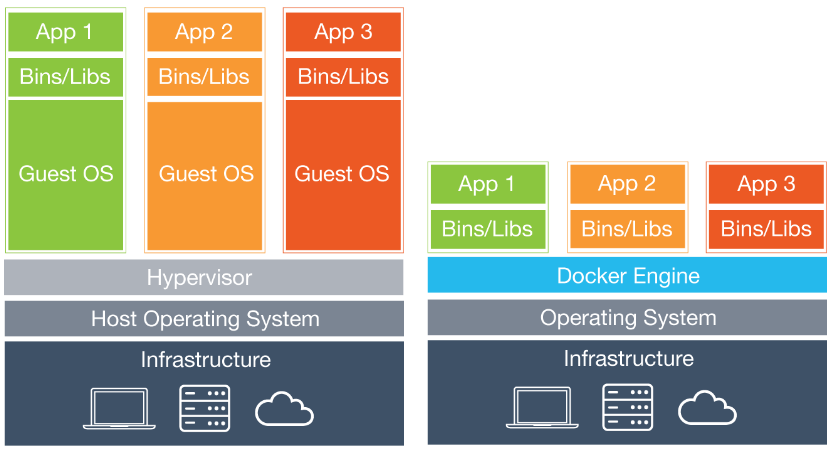
\includegraphics[width=1\linewidth]{./informe/introduccion/img/docker/vm_vs_docker}
		\caption{Contenedor Docker (derecha) versus M�quina Virtual (izquierda)
		\cite{WhatIsDocker2016}}
	\end{figure}

	Mediante el uso de contenedores, los recursos pueden ser aislados y los servicios
	restringidos. Adem�s, se otorga a los procesos la capacidad de tener una visi�n
	casi completamente privada del sistema operativo con su propio identificador de
	espacio de proceso, estructura del sistema de archivos e interfaces de red.
	Contenedores m�ltiples comparten el mismo n�cleo, pero cada contenedor puede ser
	restringido a utilizar s�lo una cantidad definida de recursos como CPU, memoria y
	E/S.\cite{WikipediaDocker}
	
	Usando Docker para crear y gestionar contenedores se puede simplificar la
	creaci�n de sistemas altamente distribuidos, permitiendo m�ltiples aplicaciones
	funcionar de forma aut�noma en una �nica m�quina f�sica o en varias m�quinas
	virtuales. Esto permite que el despliegue de nodos se realice a medida que se
	dispone de recursos o cuando se necesiten, lo que se conoce como un estilo de
	desplieque \emph{Plataforma como Servicio} (\emph{PaaS - Plataform as a
	Service}).\cite{WikipediaDocker}

	\subsection{Im�genes y Contenedores}
	
		Un \emph{contenedor (container)} es una version de un sistema operativo Linux,
		solo con los componentes m�s b�sicos. Una \emph{imagen} es software que se carga
		dentro del contenedor al momento de ejecutar el comando \emph{run}.
		\cite{GetStartedDocker2016}
	
\lstset{language=bash}
\begin{lstlisting}
docker run hello-world
\end{lstlisting}
	
		El comando \emph{run} recibe como par�metro requerido el nombre de la imagen que
		se desea cargar en un contenedor, en �ste caso, \emph{hello-world}.
		
		Al correr dicho comando, Docker ejecuta las siguientes acciones:
		\begin{itemize}
		    \item Comprobar si existe en el sistema una imagen con el nombre
		    \emph{hello-world}.
		    \item En caso de que no exista dicha imagen en el sistema descargarla desde
		    el repositorio de im�genes configurado, por defecto es \emph{Docker Hub}, un
		    repositorio propiedad de Docker donde existen miles de im�genes disponibles.
		    Es posible tener repositorios privados utilizando lo que se conoce como
		    \emph{Docker Registry}.
		    \item Cargar la \emph{imagen} en el \emph{contenedor} y ejecutarla.
		\end{itemize}
		
		Por otro lado, una imagen de Docker puede ejecutar desde un simple comando hasta
		cargar un complejo sistema de base de datos.
		
		Para construir una imagen de Docker, es necesario crear un archivo llamado
		\emph{Dockerfile}.
	
\lstset{language=bash}
\begin{lstlisting}
FROM ubuntu:16.04

RUN apt-get -y update

CMD["echo Hola"]
\end{lstlisting}
	
		El Dockerfile anterior buscara una imagen de Ubuntu con la etiqueta (\emph{tag})
		\emph{16.04}. Luego ejecutar� un comando para actualizar los paquetes del
		sistema operativo y finalmente mostrar� el mensaje \emph{Hola}.
	
		El comando para construir una \emph{imagen} de Docker es:

\lstset{language=bash}
\begin{lstlisting}
docker build -t miimagen .
\end{lstlisting}

		Se ejecutar� el comando \emph{build} para construir la imagen. El argumento
		\emph{-t} indica que se le pondr� la etiqueta \emph{miimagen} a la imagen y
		punto al final indica el directorio de contexto de la \emph{imagen}, esto
		permite agregarle archivos al momento de construirla. En �ste caso, el contexto
		ser� el directorio donde se encuentra el Dockerfile.
	
		Luego, es posible cargar la \emph{imagen} en un \emph{contenedor} mediante el
		comando:
	
\lstset{language=bash}
\begin{lstlisting}
docker run miimagen
\end{lstlisting}

	\subsection{Crear nuevas etiquetas}
	
		Para ponerle una nueva etiqueta a una imagen, primero debemos encontrar el
		n�mero de identificaci�n de la misma. �sto se hace corriendo el comando:

\lstset{language=bash}
\begin{lstlisting}
docker images
\end{lstlisting}

		El comando anterior, mostrar� una lista de las im�genes existentes en el sistema
		mostrando la �ltima etiqueta de la misma, el n�mero de identificaci�n, la fecha
		de creaci�n y el tama�o de la imagen.
		
		Luego, para aplicarle una nueva etiqueta, se ejecuta el comando:
	
\lstset{language=bash}
\begin{lstlisting}
docker tag <IMAGE_ID> <NUEVA_ETIQUETA>
\end{lstlisting}	
	
	\subsection{Docker Compose}
	
		Docker Compose es una herramienta que permite correr un sistema formado por
		m�ltiples contenedores. Para ello, se debe crear un archivo \emph{.yml} en el
		que se definan los servicios con los que va a contar la aplicaci�n. Cada
		servicio estar� formado por un \emph{contenedor} corriendo una \emph{imagen} de
		Docker.
		
		Para cada servicio pueden definirse nombres, puertos expuestos, conexiones de
		red, etc�tera, luego, con los siguientes comandos se puede operar con el sistema.
		
		Para una lista completa de los comandos de Docker Compose, acceder a \emph{Docker Compose
		Command-Line Reference}\footnote{https://docs.docker.com/compose/reference/}.

	\subsection{Material}
	
		La informaci�n de �sta secci�n ha sido extra�da mayormente desde la
		documentaci�n de Docker\cite{GetStartedDocker2016} y Docker
		Compose\cite{DockerComposeDocumentation}.
		
\section{Apache Zookeeper}
\label{section_apache_zookeeper}

	Apache Zookeeper es un servicio de coordinaci�n de alto rendimiento para
	aplicaciones distribuidas. Expone servicios comunes, tales como nomenclatura,
	manejo de las configuraciones, sincronizaci�n, etc�tera. 
	Entre otras funciones, se utiliza para implementar consenso, manejar grupos,
	elecci�n de nodo l�der y protocolos de presencia.
	
	Generalmente, los sistemas de coordinaci�n son muy propensos a errores como
	condiciones de carrera y puntos muertos (\emph{deadlocks}). Zookeeper fue creado
	para que las aplicaciones distribuidas ya no necesiten implementar desde cero los
	servicios de sincronizaci�n.
	
	\begin{figure}[H]
		\centering
		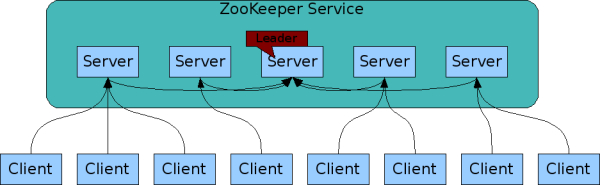
\includegraphics[width=1\linewidth]{./informe/introduccion/img/zookeeper/ZookeeperService}
		\caption{Arquitectura de un servicio Zookeeper\cite{Zookeeper348}}
	\end{figure}
	
	De acuerdo a la documentaci�n de Zookeeper, fu� dise�ado bajo estos cuatro
	pilares\cite{Zookeeper348}:
	\begin{itemize}
	    \item \emph{simplicidad}: Zookeeper permite la sincronizaci�n entre procesos
	    distribuidos a trav�s de un espacio de nombres jer�rquico compartido que se
	    encuentra organizado de manera similar a un sistema de archivos. El espacio
	    de nombres consiste en registros de datos (llamados \emph{znodes}) muy
	    similares a archivos y directorios.
	    \item \emph{replicaci�n}: Como las aplicaciones distribuidas que coordina,
	    Zookeeper tambi�n esta dise�ado para ser ejecutado de manera distribuida en
	    un conjunto de servidores. Cada uno de ellos mantiene en memoria una imagen
	    de estado con los registros de las transacciones y adem�s, guarda capturas en
	    un almacenamiento permanente. Mientras la mayor�a de los servidores siga
	    funcionando, Zookeeper seguir� funcionando.
	    
	    Cada cliente, se conecta a un �nico servidor de Zookeeper y mantiene una
	    conexi�n TCP a trav�s de la cual env�a solicitudes, obtiene las respuestas y
	    obtiene mensajes de eventos. Si dicha conexi�n deja de funcionar, el cliente
	    se conectar� a un servidor distinto.
	    \item \emph{orden}: Cada actualizaci�n en Zookeeper es marcada con un n�mero
	    que refleja el orden de cada una de las transacciones.
	    \item \emph{rapidez}: Zookeeper es muy r�pido para entornos con cargas de
	    trabajo de muchas lecturas. Su rendimiento es mucho mejor donde las lecturas
	    de datos son m�s comunes a las escrituras de datos, a una relaci�n de 10 a 1.
 	\end{itemize}
 	
 	\begin{figure}[H]
		\centering
		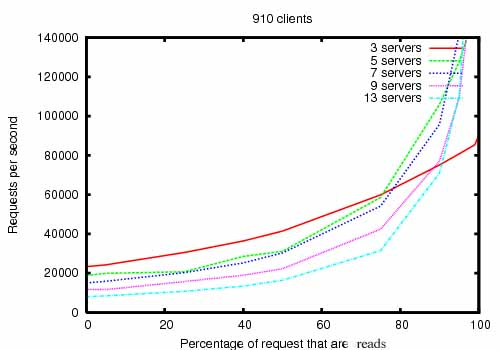
\includegraphics[width=.8\linewidth]{./informe/introduccion/img/zookeeper/ZookeeperPerformanceRW}
		\caption{Rendimiento de Zookeeper mostrando escrituras
		versus lecturas\cite{Zookeeper348}}
	\end{figure}
	
	\subsection{El espacio de nombres y el modelo de datos}
		
		El espacio de nombres de Zookeeper es muy similar a un sistema de archivos. Cada
		nombre es una secuencia de elementos de direcciones (\emph{paths}) separadas por
		una barra (\emph{/}) y cada nodo es identificado por una direcci�n.
				
		\begin{figure}[H]
			\centering
			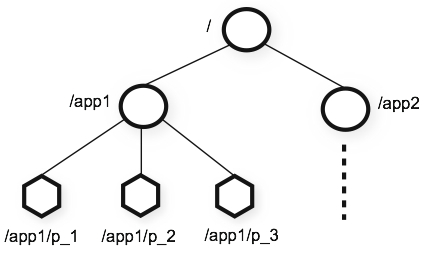
\includegraphics[width=1\linewidth]{./informe/introduccion/img/zookeeper/ZookeeperNamespace}
			\caption{El espacio de nombres jer�rquico de Zookeeper\cite{Zookeeper348}}
		\end{figure}
		
		A diferencia de los sistemas de archivos, cada nodo en el espacio de nombres de
		Zookeeper puede tener datos y subnodos, es como si un sistema de archivos
		permitiera a un archivo ser a la vez un directorio. Debido a los objetivos por
		lo cuales Zookeeper fue dise�ado, los datos almacenados en cada nodo generalemente
		son muy peque�os, en el orden de un byte a un kilobyte. Cada nodo de datos, en
		la nomenclatura de Zookeeper es llamado \emph{znode}.

		Los \emph{znodes} mantienen una estructura de datos que incluye numeros de
		version para cada cambio en los datos y marcas de tiempo para permitir
		validaciones de cache y actualizaciones coordinadas. Con cada cambio, el n�mero
		de versi�n aumenta.
		
		Los datos de cada \emph{znode} son escritos y le�dos de manera at�mica. Las
		lecturas devuelven todos los datos asociados al \emph{znode} y las escrituras
		reemplazan todos los datos. Cada nodo, tambi�n, posee una lista de control de
		acceso (\emph{ACL, Access Control List}) que limita quienes pueden ejecutar cada
		una de las acciones.
		
	\subsection{Garant�as}
	
		Dado que el objetivo de Zookeeper es ser la base para la construcci�n de
		servicios complejos, como un servicio de sincronizaci�n, provee un conjunto de
		garant�as:
		\begin{itemize}
		    \item \emph{Consistencia Secuencial}: Todas las actualizaciones que llegan
		    desde los clientes, ser�n aplicadas en el orden en el que fueron enviadas.
		    \item \emph{Atomicidad}: Las actualizaciones son exitosas o fallidas. No
		    existen resultados parciales.
		    \item \emph{�nica Imagen del Sistema}: Un cliente tiene la misma vista del
		    servicio Zookeeper sin importar a cual de los servidores se conecte.
		    \item \emph{Confiabildad}: Una vez que una actualizaci�n es aplicada,
		    persiste en el tiempo hasta que alg�n cliente sobreescribe el registro.
		    \item \emph{Actualizaciones puntuales}: El sistema garantiza a los clientes
		    que su vista del servicio estar� actualizada dentro de un cierto espacio
		    temporal.
		\end{itemize}
		
	\subsection{Material}
	
		La informaci�n de �sta secci�n ha sido extra�da mayormente desde la
		documentaci�n de Apache Zookeeper\cite{Zookeeper348}.
	
\section{Apache Kafka}
\label{section_apache_kafka}

	Kafka es un sistema de mensajes distribuido, particionado y con
	replicaci�n\cite{ApacheKafka090}.

	\begin{itemize}
	    \item Kafka mantiene los mensajes agrupados en categor�as llamadas
	    \emph{topics.}
		\item Los productores de mensajes se llaman \emph{producers}.
		\item Los consumidores de mensajes se llaman \emph{consumers}.
		\item Kafka corre en un cluster formado por uno o mas servidores. Cada uno de
		ellos es llamado \emph{broker}.
	\end{itemize}
	
	\begin{figure}[H]
		\centering
		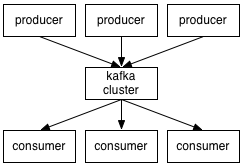
\includegraphics[width=.5\linewidth]{./informe/introduccion/img/kafka/high_level_arch}
		\caption{Kafka, arquitectura de alto nivel\cite{ApacheKafka090}}
	\end{figure}

	\subsection{Topics}
	
		Los \emph{topics} de Kafka son categor�as de mensajes para los cuales Kafka
		mantiene registros particionados.
		
		Cada partici�n es una secuencia ordenada e inmutable de mensajes. El n�mero de
		orden de cada mensaje es llamado \emph{offset} e identifica un�vocamente a cada
		mensaje de la partici�n.
		
		Kafka mantiene los mensajes publicados por un per�odo de tiempo configurable,
		sin importar si fueron consumidos o no por alg�n proceso \emph{consumer}. Cada
		consumidor se encarga de mantener el \emph{offset} y tiene libertad para ir
		hacia atr�s y hacia adelante en los mensajes publicados para procesarlos.
		
		Tener los mensajes de un \emph{topic} particionados permite separar el
		\emph{topic} en varios servidores. �sto permite manejar grandes volumenes de
		datos y adem�s otorogar un nivel superior de paralelismo.
		
		\begin{figure}[H]
			\centering
			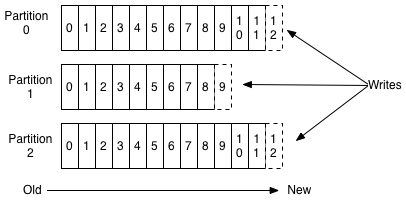
\includegraphics[width=.5\linewidth]{./informe/introduccion/img/kafka/kafka_topics}
			\caption{Topics en Kafka\cite{ApacheKafka090}}
		\end{figure}
		
		Cada partici�n est� formada por un l�der (\emph{leader}) que se encuentra en
		uno de los servidores y por cero o m�s seguidores (\emph{followers}) que
		replican al l�der todo el tiempo en servidores distintos. Si el l�der falla,
		alguno de los seguidores se convertir� en el nuevo l�der garantizando que el
		sistema siga operando. La configuraci�n ideal es que cada servidor sea l�der de
		alguna partici�n y seguidor de las otras.
		
	\subsection{Productores}
		
		Los productores en Kafka son programas encargados de publicar datos en los
		\emph{topics}. El productor decide, para cada mensaje, el \emph{topic} y la
		\emph{partici�n} en el cual publicarlo. Generalmente la partici�n es elegida
		siguiendo un esquema \emph{round-robin} para lograr un �ptimo balance de carga
		entre particiones, pero se puede utilizar cualquier l�gica.
		
	\subsection{Consumidores}
	
		Los sitemas de mensajer�a pueden ser clasificados en dos categor�as,
		\emph{cola de mensajes} o \emph{publicaci�n-subscripci�n}. En el primero, los
		mensajes son encolados y cada mensaje es dirigido hacia alguno de los
		consumidores. En el segundo, cada mensaje es transmitido a todos los
		consumidores. Apache Kafka maneja ambos mundos con lo que se conoce como
		grupos de consumidores (\emph{consumer groups}).
		
		Cada consumidor debe ubicarse dentro de alguno de los grupos de consumidores y
		cuando un mensaje es publicado en un \emph{topic}, es transmitido a un �nico
		consumidor de cada uno de los grupos de consumidores.
		
		\begin{figure}[H]
			\centering
			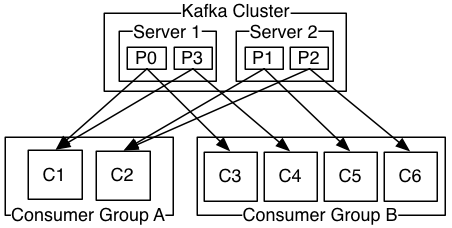
\includegraphics[width=.5\linewidth]{./informe/introduccion/img/kafka/kafka_consumers}
			\caption{Grupos de Consumidores\cite{ApacheKafka090}}
		\end{figure}
		
		Si todos los consumidores se encuentran en el mismo grupo, el sistema funciona
		como una cola de mensajes distribuyendo la carga entre cada uno de los
		consumidores.
		
		Si todos los consumidores se encuentran en distintos grupos, el sistema
		funciona como un sistema publicaci�n-subscripci�n y todos los mensajes son
		transmitidos a todos los consumidores.
		
	\subsection{Material}
	
		La informaci�n de �ste cap�tulo ha sido extra�da mayormente desde la
		documentaci�n de Apache Kafka 0.9 \cite{ApacheKafka090}.
		
\section{Apache Storm}
\label{section_apache_storm}
	
	Apache Storm es una herramienta de procesamiento de datos en tiempo real de
	c�digo abierto y gratuita creada por Twitter y luego liberada bajo la �rbita de
	los proyectos Apache.
	
	La finalidad de Storm es proveer un mecanismo confiable para procesamiento de
	flujos de datos ilimitados, haciendo para flujos de datos (\emph{realtime stream
	processing}) lo que Hadoop hace en procesamiento por lotes (\emph{batch processing})\cite{ApacheStorm097}.
	
	De acuerdo a su documentaci�n, Storm es capaz de procesar un mill�n de tuplas
	de datos por segundo por nodo. Provee caracter�sticas de escalabilidad, tolerancia a
	fallos, garant�as de que todos los datos ser�n procesados, etc�tera\cite{ApacheStorm097}.
	
	\subsection{Conceptos B�sicos}
	
		En �sta secci�n se analizar�n los conceptos b�sicos que definen a un programa
		Storm.
		
		\begin{figure}[H]
			\centering
			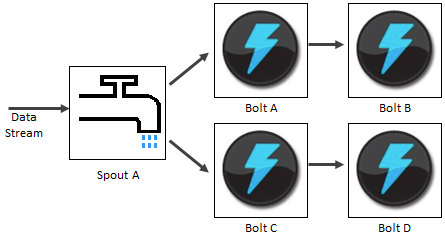
\includegraphics[width=.9\linewidth]{./informe/introduccion/img/storm/topology}
		\end{figure}
		
		\subsubsection{Topologies}
		\label{storm_topologies}
			Las \emph{topolog�as} son los contenedores de la l�gica de una aplicaci�n de
			procesamiento de datos en tiempo real en Storm. Consumen flujos de datos, los
			procesan y generan nuevos flujos de datos. Es el an�logo a un trabajo de
			MapReduce de Hadoop\footnote{https://hadoop.apache.org/docs/current/hadoop-mapreduce-client/hadoop-mapreduce-client-core/MapReduceTutorial.html}.
			La diferencia principal con �stos �ltimos es que un trabajo MapReduce de
			Hadoop, eventualmente concluye mientras que las topolog�as pueden correr
			indefinidamente. 
			Una topolog�a es un grafo formado por \emph{Spouts} y \emph{Bolts} conectados a
			trav�s de \emph{Stream Groupings} (\ref{storm_stream_grouping}).
		
		\subsubsection{Streams}
		\label{storm_streams}
			Los streams son una secuencia ilimitada de tuplas de datos que son creadas y
			procesadas de manera distribuida. Los streams se definen creando un esquema
			que contenga todos los campos de datos de cada tupla que forma parte del
			stream. Las tuplas pueden contener valores enteros (\emph{integer}), bytes,
			cadenas de caracteres (\emph{strings}), valores booleanos, etc�tera.
		
		\subsubsection{Spouts}
		\label{storm_spouts}
			Los spouts son la fuente de streams para la topolog�a. Generalemente leen
			tuplas de datos desde una fuente externa y las emiten dentro de la topolog�a
			para que sea procesada. Los spouts pueden ser:
			\begin{itemize}
			    \item \textbf{reliable} (confiable): es un spout capaz de reenviar una
			    tupla si Storm fall� en procesarla.
			    \item \textbf{unreliable} (no confiable): el spout \emph{se olvida} de las
			    tuplas en el momento en el que las emite hacia la topolog�a.
			\end{itemize}
		
		\subsubsection{Bolts}
		\label{storm_bolts}
			Dentro de una topolog�a, todo el procesamiento sobre los datos es realizado en
			los bolts. Los bolts pueden ser programados para realizar cualquier tarea como
			filtrado, agregaci�n, uniones con bases de datos, funciones, etc�tera.
			Los bolts reciben uno o varios streams de datos y pueden emitir nuevamente uno
			o varios de ellos luego de procesados.
	
		\subsubsection{Stream Grouping}
		\label{storm_stream_grouping}
			Al definir una topolog�a, es necesaria especificar que streams debe recibir
			como entrada cada uno de los bolts. Los \emph{stream groupings} definen como
			los streams deben ser particionados en las tareas de cada bolt.
			
			Existen ocho \emph{stream groupings} predefinidos pero existe la posibilidad
			de crear nuevos implementando la interfaz \emph{CustomStreamGrouping}.
			\begin{itemize}
			    \item \emph{Shuffle grouping}: Las tuplas son distribuidas aleatoriamente
			    en las tareas de los bolts de manera tal que se garantice que todos los
			    bolts reciben las misma cantidad de tuplas.
			    
			    \item \emph{Fields grouping}: El stream es particionado de acuerdo a los
			    campos de datos que contenga la tupla. Por ejemplo, si la tupla contiene
			    un campo llamado \emph{usuario} y se agrupa el stream por el campo
			    \emph{usuario}, todos aquellas tuplas que tengan el mismo valor en dicho
			    campo ser�n procesadas por el mismo bolt.
			    
			    \item \emph{Partial Key grouping}: El stream es particionado de la misma
			    manera que en el caso de \emph{Fields grouping} solo que la carga es
			    balanceada entre dos bolts para proporcionar una mejor utilizaci�n de los
			    recursos.
			    
			    \item \emph{All grouping}: El stream de datos es replicado en TODAS las
			    tareas de los bolts.
			    
			    \item \emph{Global grouping}: El stream completo es dirigido hacia una
			    �nica tarea de un bolt.
			    
			    \item \emph{None grouping}: Al utilizar esta forma de agrupamiento, se
			    est� indicando que no es importante como el stream es dirigido hacia los
			    bolts.
			    
			    \item \emph{Direct grouping}: En �ste caso, el productor de la tupla de
			    datos decide a que tarea del bolt consumidor desea enviar la tupla.
			    
			    \item \emph{Local grouping}: Si el bolt de destino tiene una o m�s tareas
			    en el mismo proceso \emph{worker}, las tuplas ir�n aleatoriamente hacia
			    alquellas tareas que est�n siendo ejecutadas. En caso contrario, se
			    comportar� como un \emph{Shuffle grouping}.
			\end{itemize}
	
		\subsubsection{Tasks}
		\label{storm_tasks}
			Cada spout o bolt ejecuta sus tareas en el cluster de Storm. Cada tarea
			corresponde con un hilo de ejecuci�n (\emph{thread}) y los \emph{Stream
			groupings} definen como las tuplas viajan entre las tareas.
			
		\subsubsection{Workers}
		\label{storm_workers}
			Las topolog�as corren sobre uno o m�s procesos \emph{worker}. Cada uno de
			estos procesos es una JVM que ejecuta un subconjunto de las tareas de
			la topolog�a.
		
	\subsection{Material}
	
		La informaci�n de �ste cap�tulo ha sido extra�da mayormente desde la
		documentaci�n de Apache Storm 1.0 \cite{ApacheStorm097}.

 		% Desarrollo
 			\part{Desarrollo}
 				% Dise�o de la Arquitectura del Sistema
 					%%%%%%%%%%%%%%%%%%%%%%%%%%%%%%%%%%%%%%%%%%%%%%%%%%%%%%%%%%%%%%%%%%%%%%%%%%%%%%%%%
%																				%
%	TRABAJO:	Trabajo Final													%
%				Especialidad en Ingenier�a en Sistemas de Informaci�n			%
%																				%
%		Titulo:	Procesamiento de Datos en Tiempo Real							%
%																				%
%		Autor:	Juli�n Nonino													%
%																				%
%	Dise�o de la Arquitectura del Sistema										%	
%																				%
%	A�o: 2016																	%
%																				%
%%%%%%%%%%%%%%%%%%%%%%%%%%%%%%%%%%%%%%%%%%%%%%%%%%%%%%%%%%%%%%%%%%%%%%%%%%%%%%%%%

\chapter{Dise�o de la Arquitectura del Sistema}
\label{chapter_arquitectura}

Para cumplir con el objetivo de armar un sistema de procesamiento de dato en
tiempo real utilizando tecnolog�as como Docker, Apache Zookeeper, Apache Kafka y
Apache Storm. Se plantea un sistema multinodo, con cada nodo corriendo un
determinado servicio basado en la imagen de Docker generada.

Como se observa en la figura \ref{arquitectura_general}, se generar�n
tres nodos de Apache Zookeeper, al igual que con Apache Kafka. Esto permite
garantizar la disponibiliad de los servicios. En el caso de Apache Storm, se
generan tres nodos, uno para el procesamiento de datos (podr�an existir m�s), un
�nico nodo encargado de controlar el cl�ster, \emph{Storm Nimbus}, y un nodo
adicional para acceder a la interfaz gr�fica de Apache Storm.

\begin{figure}[H]
	\centering
	\label{arquitectura_general}
	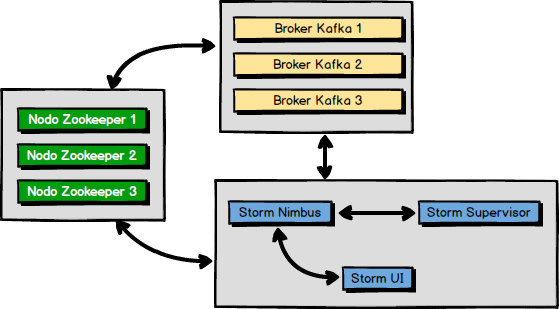
\includegraphics[width=1\linewidth]{./informe/desarrollo/img/ArquitecturaServidor}
	\caption{Arquitectura general del Cl�ster incluyendo Zookeeper, Kafka y Storm}
\end{figure}

\newpage

Tambi�n, se implementan dos simples aplicaciones en Java. Una, para actuar de
productor de datos para Apache Kafka, simulando alg�n dispositivo o sistema que
env�a datos al servidor. La otra es la topolog�a de Apache Storm encargada de
leer los datos desde Apache Kafka y efectuarles alg�n procesamiento. �sta
topolog�a, ser� subida al nodo \emph{Storm Nimbus}.

\begin{figure}[H]
	\centering
	\label{arquitectura general_clientes}
	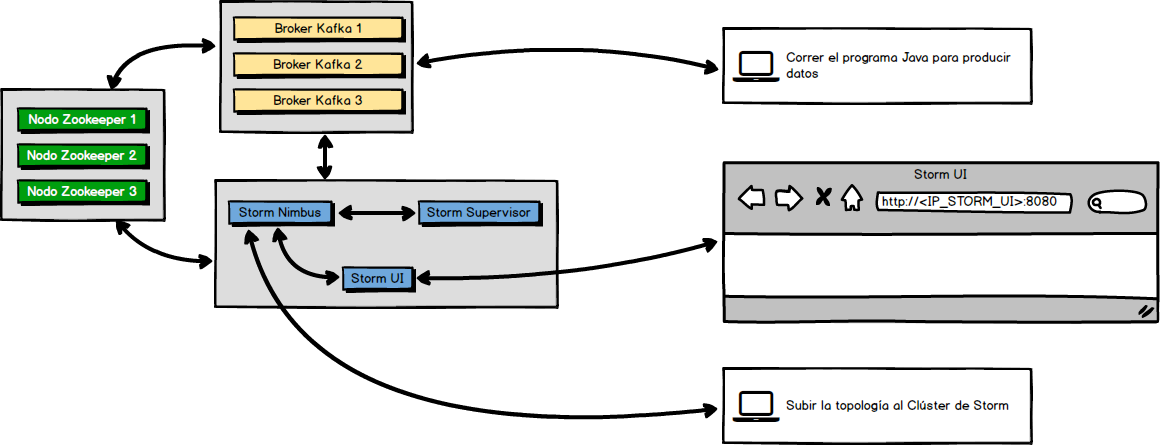
\includegraphics[width=1\linewidth]{./informe/desarrollo/img/ArquitecturaConexionClientes}
	\caption{Arquitectura general del Cl�ster conectado a los programas cliente}
\end{figure}

 				% Im�genes de Docker
 					%%%%%%%%%%%%%%%%%%%%%%%%%%%%%%%%%%%%%%%%%%%%%%%%%%%%%%%%%%%%%%%%%%%%%%%%%%%%%%%%%
%																				%
%	TRABAJO:	Trabajo Final													%
%				Especialidad en Ingenier�a en Sistemas de Informaci�n			%
%																				%
%		Titulo:																	%
%																				%
%		Autor:	Juli�n Nonino													%
%																				%
%	Capitulo sobre las im�genes de Docker Creadas								%	
%																				%
%	A�o: 2016																	%
%																				%
%%%%%%%%%%%%%%%%%%%%%%%%%%%%%%%%%%%%%%%%%%%%%%%%%%%%%%%%%%%%%%%%%%%%%%%%%%%%%%%%%

\lstset
{	basicstyle=\tiny,       		% the size of the fonts that are used for the code
	numbers=left,                   % where to put the line-numbers
	numberstyle=\tiny\color{gray},  % the style that is used for the line-numbers
	stepnumber=1,                   % the step between two line-numbers. If it's 1, each line will be numbered
	numbersep=5pt,                  % how far the line-numbers are from the code
	showspaces=false,               % show spaces adding particular underscores
	showstringspaces=false,         % underline spaces within strings
	showtabs=false,                 % show tabs within strings adding particular underscores
	frame=none,                 	% adds a frame around the code
	rulecolor=\color{white},        % if not set, the frame-color may be changed on line-breaks within not-black text (e.g. comments (green here))
	tabsize=2,                      % sets default tabsize to 2 spaces
	captionpos=b,                   % sets the caption-position to bottom
	breaklines=true,                % sets automatic line breaking
	breakatwhitespace=true,        	% sets if automatic breaks should only happen at
	keywordstyle=\color{blue},     	% keyword style
  	commentstyle=\color{dkgreen}, 	% comment style
  	stringstyle=\color{gray},      	% string literal style
  	escapeinside={\%*}{*)},         % if you want to add LaTeX within your code
  	morekeywords={*,apt-get,...},   % if you want to add more keywords to the set
  	deletekeywords={local,...}      % if you want to delete keywords from the given language
}

\chapter{Im�genes de Docker}
\label{chapter_docker_images}

El sistema desarrollado se compone de una serie de im�genes de Docker que al
ejecutarse como Docker Containers, formar�n el sistema de procesamiento de datos
en tiempo real que se quiere demostrar. Las im�genes desarrolladas son:

\begin{itemize}
    \item Nodo de Apache Zookeeper (\ref{docker-image-nodo-zookeeper}).
    \item Nodo de Apache Kafka (\ref{docker-image-nodo-kafka}).
    \item Imagenes de Apache Storm (\ref{docker-images-storm}).
    	\begin{itemize}
    	  \item Nodo de Apache Storm Nimbus (\ref{docker-images-storm-nimbus}).
    	  \item Nodo de Apache Storm
    	  Supervisor (\ref{docker-images-storm-supervisor}).
    	  \item Nodo de Apache Storm UI (\ref{docker-images-storm-ui}).
		\end{itemize}
\end{itemize}

\begin{figure}[H]
	\centering
	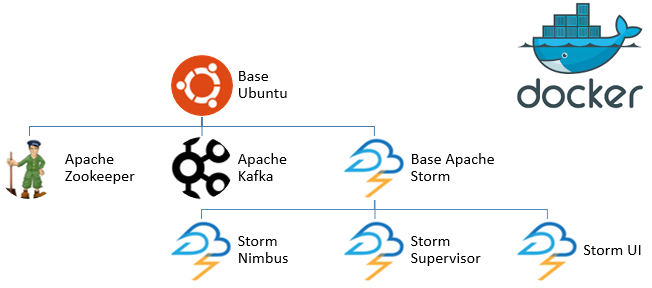
\includegraphics[width=1\linewidth]{./informe/desarrollo/img/JerarquiaImagenesDocker}
	\caption{Jerarqu�a de las im�genes de Docker desarrolladas}
\end{figure}
	
\section{Nodo Apache Zookeeper}
\label{docker-image-nodo-zookeeper}

	Basado en una imagen de Ubuntu 14.04 Trusty, se desarrolla la imagen de
	Apache Zookeeper.

	\lstinputlisting[language=Bash,
					 caption={Dockerfile para un nodo de Apache Zookeeper},
					 label=code_zookeeper_dockerfile
					]{./docker_images/zookeeper/Dockerfile.}
	
	Para comenzar, se realiza una actualizaci�n del sistema operativo y luego se
	procede con la instalaci�n de Apache Zookeeper a trav�s de la
	herramienta \emph{apt-get} de Ubuntu. Luego, se limpian todos los restos que
	hayan quedado de la instalaci�n para reducir el tama�o de la imagen.
	Posteriormente, se exponen los puertos necesarios para la ejecuci�n.
	
	Con eso ya se podr�a iniciar un �nico nodo de Apache Zookeeper agregando a la
	imagen el siguiente comando.
	
\lstset{language=Bash}
\begin{lstlisting}
CMD ["/usr/share/zookeeper/bin/zkServer.sh", "start-foreground"]
\end{lstlisting}

	Como se desea correr un cl�ster de Apache Zookeeper, se deben hacer ciertas
	configuraciones para que cada nodo pueda comunicarse con los dem�s. Por �sta
	raz�n se implementa el siguiente script de inicio.
	
	\lstinputlisting[language=Bash,
					 caption={Script de inicio para un nodo de Apache Zookeeper},
					 label=code_zookeeper_start_sh
					]{./docker_images/zookeeper/start.sh}

	Lo que hace el script \ref{code_zookeeper_start_sh} es recibir como par�metros
	una identificaci�n para el nodo y una lista de todos los nodos y configura Apache
	Zookeeper con esos datos antes de iniciar el servicio. Se hace de �sta manera
	debido al alcance de �sta demostraci�n, en producci�n deber�a utilizarse alg�n
	sistema de auto descubrimiento de servicios para que los nodos se encuentren
	autom�ticamente al levantarse.

	La construcci�n de �sta imagen, se realiza situado en la carpeta
	\emph{zookeeper} del repositorio, mediante el siguiente comando.
	
\lstset{language=Bash}
\begin{lstlisting}
docker build -t jnonino/zookeeper .
\end{lstlisting}
	\newpage
	Luego de construir la imagen de Zookeeper, el cl�ster de tres nodos puede ser
	lanzado mediante Docker Compose utilizando el siguiente comando:

\lstset{language=Bash}
\begin{lstlisting}
docker-compose -f start_zookeeper.yml up -d
\end{lstlisting}
	
	El comando anterior	inicia tres nodos de Zookeeper basados en la imagen
	construida anteriormente, el valor \emph{-d} al final indica que se desea que
	los containers corran en segundo plano.
	
	\lstinputlisting[language=Bash,
					 caption={Script de inicio de Docker Compose para levantar un cl�ster de
					 3 nodos de Apache Zookeeper},
					 label=code_zookeeper_compose
					 ]{./docker_images/zookeeper/start_zookeeper.yml}
	
	Notar que se utiliza la misma direcci�n IP para los tres nodos, �sto se debe a
	que para la demostraci�n que se hace en �ste trabajo, todos los servicios
	correran en un mismo servidor. L�gicamente, en un sistema en producci�n,
	atendiendo datos de clientes, dichos servicios deber�an correr en instancias
	diferenciadas para garantizar la alta disponibilidad que Apache Zookeeper promete
	al utilizar m�s de un nodo.
	
	Para comprobar que los tres nodos est�n corriendo correctamente, ejecutar el
	siguiente comando:

\lstset{language=Bash}
\begin{lstlisting}
for i in {2181..2183}; do 
	echo mntr | nc <IP_DEL_HOST> $i | grep zk_followers ;
done
\end{lstlisting}	

	Se debe obtener un resultado como el siguiente mostrando que Zookeeper est�
	corriendo y que hay dos nodos adem�s del nodo l�der.

\lstset{language=Bash}
\begin{lstlisting}
zk_followers	2
\end{lstlisting}

\section{Nodo de Apache Kafka}
\label{docker-image-nodo-kafka}

	De la misma manera que los nodos de Apache Zookeeper, �sta imagen es basada en la
	imagen Ubuntu 14.04 Trusty. Y, como primera medida, se procede a la actualizaci�n
	del sistema operativo.

	\lstinputlisting[language=Bash,
					 caption={Dockerfile para un nodo de Apache Kafka},
					 label=code_kafka_dockerfile
					]{./docker_images/kafka/Dockerfile.}
	
	En �ste caso, se proceden a instalar herramientas como \emph{wget}, \emph{tar} y
	\emph{Java 7 JRE} necesarias para que corra Apache Kafka. Debido a que Kafka no
	puede ser instalado mediante \emph{apt-get}, es necesario descargar el archivo
	\emph{.tar}, descomprimirlo y ejecutarlo.
	
	Luego de configurar el nodo, es posible lanzar Kafka mediante un script utilizado
	para configurar variables antes de la ejecuci�n.
	
	\lstinputlisting[language=Bash,
					 caption={Script de inicio para un nodo de Apache Kafka},
					 label=code_kafka_start_sh
					]{./docker_images/kafka/start.sh}

	La construcci�n de �sta imagen, se realiza situado en la carpeta \emph{kafka} del
	repositorio, mediante el siguiente comando.
	
\lstset{language=Bash}
\begin{lstlisting}
docker build -t jnonino/kafka .
\end{lstlisting}

	Luego de construir la imagen, el cl�ster de tres nodos puede ser lanzado mediante
	Docker Compose utilizando el siguiente comando: 

\lstset{language=Bash}
\begin{lstlisting}
docker-compose -f start_kafka.yml up -d
\end{lstlisting}
	
	El comando anterior	inicia tres nodos de Kafka basados en la imagen
	construida anteriormente, el valor \emph{-d} al final indica que se desea que
	los containers corran en segundo plano.
	
	\lstinputlisting[language=Bash,
					 caption={Script de inicio de Docker Compose para levantar un cl�ster de
					 3 nodos de Apache Kafka},
					 label=code_zookeeper_compose
					 ]{./docker_images/kafka/start_kafka.yml}
	
	Notar que se utiliza la misma direcci�n IP para los tres nodos, �sto se debe a
	que para la demostraci�n que se hace en �ste trabajo, todos los servicios
	correran en un mismo servidor. L�gicamente, en un sistema en producci�n,
	atendiendo datos de clientes, dichos servicios deber�an correr en instancias
	diferenciadas para garantizar la alta disponibilidad que Apache Kafka promete
	al utilizar m�s de un nodo.
	
	Para comprobar que los tres nodos est�n corriendo correctamente, es necesario
	descargar Kafka para interactuar con el servidor corriendo\footnote{Descargar
	Apache Kafka desde https://www.apache.org Version 0.9.0.1 con Scala 2.11}.

	Correr los siguientes comandos para crear un t�pico de prueba y obtener
	informaci�n del mismo:
	
\lstset{language=Bash}
\begin{lstlisting}
./bin/kafka-topics.sh --create --topic test --partitions 3 --zookeeper
<IP_ZOOKEEPER> --replication-factor 2
./bin/kafka-topics.sh --describe --topic test --zookeeper <IP_ZOOKEEPER>
\end{lstlisting}	

	\begin{figure}[H]
		\centering
		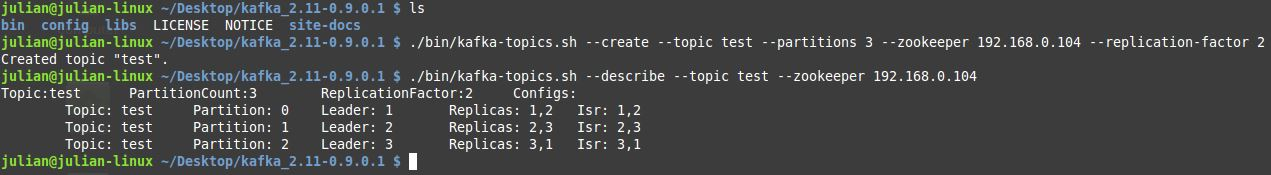
\includegraphics[width=1\linewidth]{./informe/desarrollo/img/kafka_creacion_topic}
	\end{figure}

	Para enviar datos al servidor de Kafka, se debe generar una lista de los nodos de
	Kafka (\emph{brokers}) para posteriormente enviarle mensajes y finalmente, con
	otra aplicaci�n provista por Kafka, leerlos.

\lstset{language=Bash}
\begin{lstlisting}
BROKER_LIST=<IP_NODO_KAFKA>:9092,<IP_NODO_KAFKA>:9093,<IP_NODO_KAFKA>:9094
/bin/kafka-console-producer.sh --topic test --broker-list="$BROKER_LIST"
./bin/kafka-console-consumer.sh --zookeeper <IP_ZOOKEEPER> --topic test
--from-beginning
\end{lstlisting}

	\begin{figure}[H]
		\centering
		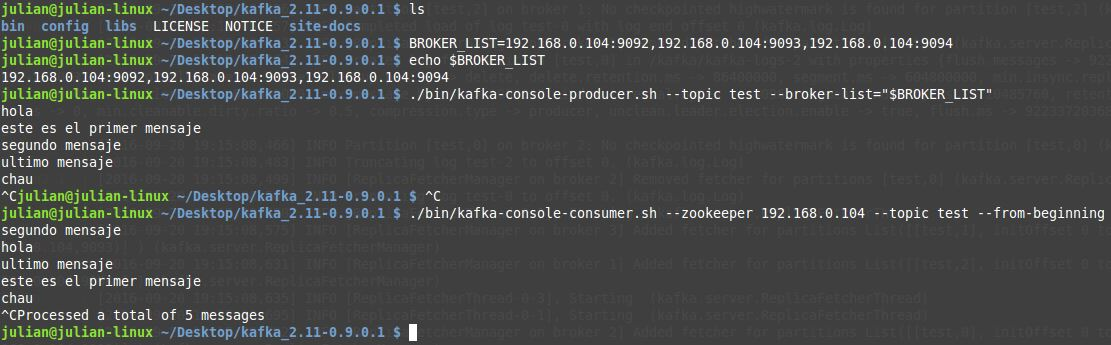
\includegraphics[width=1\linewidth]{./informe/desarrollo/img/kafka_w_r_topic}
	\end{figure}

\section{Apache Storm}
\label{docker-images-storm}

	Un cl�ster de Apache Storm necesita contar con varios tipos de nodos para su
	operaci�n. En las siguientes secciones se mostrar�n las im�genes de Docker
	creadas para cada uno de ellos y se comentar� cual es el prop�sito de dicho
	nodo.
	
	\begin{figure}[H]
		\centering
		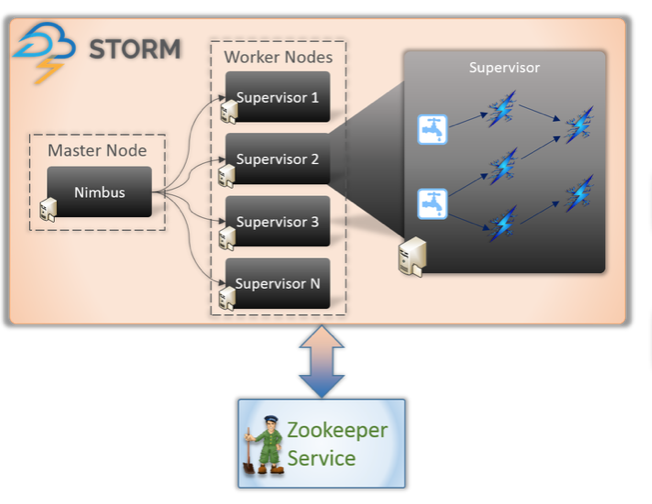
\includegraphics[width=1\linewidth]{./informe/desarrollo/img/Cluster-Storm}
		\caption{Arquitectura b�sica de un cl�ster de Apache Storm\cite{Prakash2016}}
	\end{figure}
		
	Tambi�n basada en una imagen de docker de Ubuntu 14.04 Trusty se crea la imagen
	base para todos los servicios de Storm. 
	Cada nodo de Storm debe correr dos aplicaciones \emph{storm-supervisor} y
	\emph{storm-logviewer}. Para correr ambos procesos en un container de Docker, se
	utiliza un sistema de control de procesos hecho en Python llamado
	\emph{supervisord}.
	
	Es necesario correr tres servicios, \emph{Storm Nimbus}, \emph{Storm
	UI} y al menos un nodo \emph{Storm Supervisor}. Dado que los tres compartes
	muchas configuraciones, se crea una imagen base de Apache Storm de la cual
	derivar�n los tres servicios necesarios.
	
	\lstinputlisting[language=Bash,
					 caption={Dockerfile para la imagen base de Storm},
					 label=code_storm_base_dockerfile
					]{./docker_images/storm/storm-base/Dockerfile.}

	Se comienza actualizando el sistema operativo, luego se instalan todas las
	herramientas necesarias como \emph{tar}, \emph{wget} y \emph{supervisord}. Como
	no es posible la instalaci�n de Apache Storm desde la herramienta \emph{apt-get},
	se debe realizar un procedimiento similar al seguido con Apache Kafka.
	Por �ltimo, se copian varios archivos de configuraci�n que son necesarios para la
	ejecuci�n de supervisord y Apache Storm.
	
	\lstinputlisting[language=XML,
					 caption={Archivo de configuraci�n de Apache Storm storm.yaml},
					 label=code_storm_yaml
					]{./docker_images/storm/storm-base/storm.yaml}

	\lstinputlisting[language=XML,
					 caption={Archivo de configuraci�n de Apache Storm cluster.xml},
					 label=code_cluster_xml
					]{./docker_images/storm/storm-base/cluster.xml}
	
	\lstinputlisting[language=Bash,
					 caption={Archivo de configuraci�n de SupervisorD config-supervisord.sh},
					 label=code_config_supervisord_sh
					]{./docker_images/storm/storm-base/config-supervisord.sh}
	
	\lstinputlisting[language=Bash,
					 caption={Script de inicio de Storm},
					 label=code_start_supervisor_sh
					]{./docker_images/storm/storm-base/start-supervisor.sh}
	
	\subsection{Storm Nimbus}
	\label{docker-images-storm-nimbus}
	
		Storm Nimbus, es el nodo maestro y coordinador de Apache Storm. Es el
		encargado de asignar las tareas a los nodos trabajadores (\emph{workers}),
		monitorear el cluster buscando fallas y distribuir el c�digo
		(\emph{topolog�as}) entre todos los nodos del cluster. Corre un proceso
		demonio llamado \textbf{\emph{nimbus}}.
		
		\lstinputlisting[language=Bash,
					 caption={Dockerfile para la imagen de Storm Nimbus},
					 label=code_storm_nimbus_dockerfile
					]{./docker_images/storm/storm-nimbus/Dockerfile.}
	
	\subsection{Storm Supervisor}
	\label{docker-images-storm-supervisor}
	
		Son los nodos trabajadores (\emph{workers}). Corren un proceso
		demonio llamado \textbf{\emph{supervisor}}. Son nodos que estan escuchando
		permanente al nodo nimbus esperando que les sean asignadas tareas.
	
		\lstinputlisting[language=Bash,
					 caption={Dockerfile para la imagen de Storm Supervisor},
					 label=code_storm_supervisor_dockerfile
					]{./docker_images/storm/storm-supervisor/Dockerfile.}
					
	\subsection{Storm UI}
	\label{docker-images-storm-ui}
	
		�sta im�gen de Docker es la encargada de levantar la interfaz gr�fica de
		Apache Storm.
		
		\lstinputlisting[language=Bash,
					 caption={Dockerfile para la imagen de Storm UI},
					 label=code_storm_ui_dockerfile
					]{./docker_images/storm/storm-ui/Dockerfile.}				
	
	\subsection{Iniciar Apache Storm}
	
			Finalizada la construcci�n de todas las im�genes anteriores, es posible
			poner a correr un servidor de Apache Storm utilizando el siguiente comando:

\lstset{language=Bash}
\begin{lstlisting}
docker-compose -f start_storm.yml up -d
\end{lstlisting}
	
	El comando anterior	inicia los tres servicios de Storm necesarios, Storm
	Nimbus, Storm Supervisor y Storm UI, el valor \emph{-d} al final indica que se
	desea que los containers corran en segundo plano.
	
	\lstinputlisting[language=Bash,
					 caption={Script de inicio de Docker Compose para levantar Apache Storm},
					 label=code_storm_compose
					 ]{./docker_images/storm/start_storm.yml}
	
	Luego, es posible comprobar el estado de Storm accediendo a la interfaz web
	\url{http://<DOCKER_HOST_IP>:8080}.

 				% Aplicaciones Desarrolladas
 					%%%%%%%%%%%%%%%%%%%%%%%%%%%%%%%%%%%%%%%%%%%%%%%%%%%%%%%%%%%%%%%%%%%%%%%%%%%%%%%%%
%																				%
%	TRABAJO:	Trabajo Final													%
%				Especialidad en Ingenier�a en Sistemas de Informaci�n			%
%																				%
%		Titulo:	Procesamiento de Datos en Tiempo Real							%
%																				%
%		Autor:	Juli�n Nonino													%
%																				%
%	Aplicaciones Desarrolladas													%	
%																				%
%	A�o: 2016																	%
%																				%
%%%%%%%%%%%%%%%%%%%%%%%%%%%%%%%%%%%%%%%%%%%%%%%%%%%%%%%%%%%%%%%%%%%%%%%%%%%%%%%%%

\chapter{Aplicaciones Desarrolladas}
\label{chapter_aplicaciones_desarrolladas}

En �ste cap�tulo se mostrar�n las aplicaciones desarrolladas para hacer uso del
sistema de procesamiento de datos presentado en secciones
anteriores (\ref{arquitectura_general}).

Los datos ingresan al sistema a trav�s de Apache Kafka, por ello, se comenz�
generando una aplicaci�n para enviar datos al servicio de Apache Kafka y otra
para consumirlos directmente desde Apache Kafka.

Tambi�n, se desarrollo una aplicaci�n de Apache Storm, \textbf{topolog�a}, que
recuperar� los datos del servicio de Apache Kafka teniendolos disponibles para
procesarlos en Apache Storm.

\section{Productor de Datos de Kafka}
\label{productor_kafka}

	Para generar una entrada de datos al sistema, se implement� una aplicaci�n Java
	encargada de publicar datos en Apacker Kafka. Paralelamente, se implement� una
	aplicaci�n consumidora de datos con el objetivo de comprobar que la producci�n
	de datos es correcta.

	\begin{figure}[H]
		\centering
		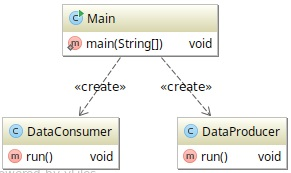
\includegraphics[width=.6\linewidth]{./informe/desarrollo/img/KafkaClassDiagram}
	\end{figure}

	Existe una clase \emph{Main} encargada de recibir los par�metros de entrada de
	la aplicaci�n e inicializar hilos de ejecuci�n productores y/o consumidores de
	datos seg�n sea necesario.

	\lstinputlisting[language=Java,
					 caption={Clase Main de la aplicaci�n de Apache Kafka},
					 label=kafka_app_main
					]{./software/kafka/src/main/java/ar/edu/utn/frc/posgrado/jnonino/kafka/Main.java}
	
	Como par�metros, se reciben la lista de brokers de Apache Kafka,
	indicadores \emph{yes|no} para habilitar el hilo productor y/o el hilo
	consumidor y finalmente, un par�metro n�merico indicando, en milisegundos, la
	tasa de producci�n de mensajes.

	\newpage

	La producci�n de datos se hacer en una clase llamada
	\emph{DataProducer} (\ref{kafka_app_producer}) que extiende de la clase
	\emph{Thread} de Java. Al momento de instanciar un objeto de �sta clase, se debe enviar la
	lista de brokers de Kafka y el valor de milisegundos que indica la tasa de
	producci�n de mensajes.

	\lstinputlisting[language=Java,
					 caption={Productor de datos de la aplicaci�n de Apache Kafka},
					 label=kafka_app_producer
					]{./software/kafka/src/main/java/ar/edu/utn/frc/posgrado/jnonino/kafka/DataProducer.java}

	El m�todo \emph{run} lee datos desde un archivo texto donde cada l�nea es un
	mensaje independiente y los publica en Apache Kafka. El formato de los
	mensajes incluye pais, provincia, ciudad, tiempo, temperatura, humedad,
	presi�n, velocidad y direcci�n del viento.
	
\lstset{language=Bash}
\begin{lstlisting}
Argentina,Catamarca,Aconquija,1207105200000,25.2,49.7,962,5.1,SUR
\end{lstlisting}

	\newpage
	
	Para el caso del consumidor de datos, se repite el mismo esquema de instanciar
	un objeto que extiende la clase \emph{Thread} de Java recibiendo como par�metro
	la lista de brokers de Kafka.
	
	En el m�todo \emph{run}, se recuperan mensajes desde el servidor y se los
	imprimi en la consola de usuario.

	\lstinputlisting[language=Java,
					 caption={Consumidor de prueba de la aplicaci�n de Apache Kafka},
					 label=kafka_app_consumer
					]{./software/kafka/src/main/java/ar/edu/utn/frc/posgrado/jnonino/kafka/DataConsumer.java}

\section{Topolog�a de Procesamiento de Datos de Storm}
\label{topologia_storm}
	
	La tolopolog�a de Apache Storm dise�ada, tiene como objetivo leer datos de
	Apache Kafka con un \emph{spout} y, un \emph{bolt} que recibir� esos datos
	imprimiendo en los registros el dato leido. Como trabajo futuro ser�a posible
	dise�ar e implementar \emph{bolts} m�s complejos para guardar los datos en una
	base de datos, implementar agregaci�n de datos para c�lculo de promedios,
	etc�tera \ref{trabjo_futuro}.
	
	\begin{figure}[H]
		\centering
		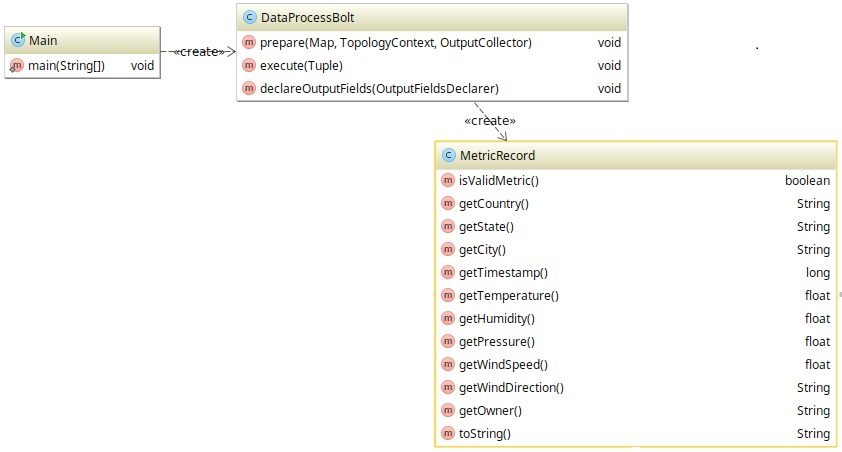
\includegraphics[width=.75\linewidth]{./informe/desarrollo/img/StormClassDiagram}
	\end{figure}
	
	La clase \emph{Main} tiene como responsabilidad recibir los par�metros el modo
	de prueba de la topolog�a, puede ser \emph{local} o \emph{cluster}. En el
	primero, la prueba se realizar� en un entorno local de Apache Storm, el
	segundo, es para utilizar la topolog�a en un entorno como el desarrollado en
	cap�tulos anteriores. Tambi�n, recibe como par�metros, la direcci�n de Apache
	Zookeeper, que ser� utilizada para encontrar las particiones de Apache Kafka
	para leer los datos.
	
	\lstinputlisting[language=Java,
					 caption={Clase Main de la topolog�a para Apache Storm},
					 label=storm_topology_main
					]{./software/storm/src/main/java/ar/edu/utn/frc/posgrado/jnonino/storm/Main.java}
					
	Dicha clase (\ref{storm_topology_main}), tambi�n es reponsable de armar el
	\emph{spout} que leer� los datos de Apache Kafka, instanciar un objeto de la
	clase \emph{DataProcessBolt} (\ref{storm_topology_bolt}) y con ambos, armar la
	topolog�a.
	
	El \emph{bolt} (\ref{storm_topology_bolt}) de procesamiento de datos, recibe
	una tupla de datos, el mensaje le�do de Apache Kafka, y registra su
	procesamiento utilizando un \emph{logger}. Luego, env�a un mensaje de
	\emph{ackowledgement} avisando que dicha tupla fue procesada.
	
	\lstinputlisting[language=Java,
					 caption={Bolt de procesamiento de datos de la topolog�a para Apache Storm},
					 label=storm_topology_bolt
					]{./software/storm/src/main/java/ar/edu/utn/frc/posgrado/jnonino/storm/DataProcessBolt.java}
	
	La clase \emph{MetricRecord} (\ref{storm_topology_metric_record}) tiene como
	objetivo representar al objeto que contiene las m�tricas recibidas en cada
	mensaje para facilitar su procesamiento.
	
	\lstinputlisting[language=Java,
					 caption={Objeto utilizado para procesar las tuplas recibidas en la
					 topolog�a para Apache Storm}, 
					 label=storm_topology_metric_record
					]{./software/storm/src/main/java/ar/edu/utn/frc/posgrado/jnonino/storm/MetricRecord.java}

 		% Resultados y Conclusiones			
 			\part{Resultados y Conclusiones}
 				% Resultados
 					%%%%%%%%%%%%%%%%%%%%%%%%%%%%%%%%%%%%%%%%%%%%%%%%%%%%%%%%%%%%%%%%%%%%%%%%%%%%%%%%%
%																				%
%	TRABAJO:	Trabajo Final													%
%				Especialidad en Ingenier�a en Sistemas de Informaci�n			%
%																				%
%		Titulo:																	%
%																				%
%		Autor:	Juli�n Nonino													%
%																				%
%	Trabajo Futuro																%	
%																				%
%	A�o: 2016																	%
%																				%
%%%%%%%%%%%%%%%%%%%%%%%%%%%%%%%%%%%%%%%%%%%%%%%%%%%%%%%%%%%%%%%%%%%%%%%%%%%%%%%%%

\chapter{Resultados}
	
 				% Conclusiones
 					%%%%%%%%%%%%%%%%%%%%%%%%%%%%%%%%%%%%%%%%%%%%%%%%%%%%%%%%%%%%%%%%%%%%%%%%%%%%%%%%%
%																				%
%	TRABAJO:	Trabajo Final													%
%				Especialidad en Ingenier�a en Sistemas de Informaci�n			%
%																				%
%		Titulo:	Procesamiento de Datos en Tiempo Real							%
%																				%
%		Autor:	Juli�n Nonino													%
%																				%
%	Conclusiones y Trabajo Futuro												%
%																				%
%	A�o: 2016																	%
%																				%
%%%%%%%%%%%%%%%%%%%%%%%%%%%%%%%%%%%%%%%%%%%%%%%%%%%%%%%%%%%%%%%%%%%%%%%%%%%%%%%%%

\chapter{Conclusiones y Trabajo Futuro}

\section{Conclusiones}
\label{conclusiones}

	En este trabajo se ha logrado implementar una prueba de concepto utilizando
	Docker como mecanismo de generaci�n de la infraestructura. Se ha mostrado c�mo
	utilizar una tecnolog�a como \emph{Apache Kafka} para recibir y reenviar
	mensajes para que sean procesados en el sistema. Tambi�n, el despliegue y
	configuraci�n de \emph{Apache Storm} para procesar dichos mensajes. Adem�s, se
	muestra el uso de \emph{Apache Zookeeper} como mecanismo de coordinaci�n entre
	estos servicios.

	Por otro lado, se muestra c�digo de aplicaciones desarrolladas para la
	publicaci�n y lectura de datos en Apache Kafka. De la misma manera, se
	implementa una topolog�a de Apache Storm para leer datos desde el servicio de
	Apache Kafka y procesarlos en tiempo real, a medida que son recibidos en el
	sistema.

	El procesamiento de flujos de datos es requerido y toma mucha relevancia cuando
	cada dato debe ser procesado r�pidamente y/o continuamente, por ejemplo, cuando
	hay que tomar acciones en tiempo real\cite{Wahner2014}, es especialmente
	importante en productos Big Data e Internet de las Cosas (\emph{Internet of
	Things}).

\section{Trabajo Futuro}
\label{trabajo_futuro}

	Este trabajo puede ser continuado y mejorado desde varias aristas, ampliando la
	prueba de concepto hasta llegar a implementar un sistema de procesamiento de
	datos en tiempo real, desplegado en la nube, con capacidad de crecer y decrecer
	de acuerdo a la carga del sistema.
	
	\begin{itemize}
	    \item Dise�ar el implementar \emph{bolts} de Apache Storm para tomar
	    \item Utilizar un proveedor de servicios en la nube como Amazon Web Services,
	    Microsoft Azure, Google Cloud Platform, etc�tera.
	    \item Plantear, implementar y probar mecanismos de auto escalabilidad
	    (crecimiento y decrecimiento) del sistema de acuerdo con la carga de datos.
	    \item Plantear, implementar y probar un subsistema de almacenamiento de datos
	    utilizando tecnolog�as bases de datos como Apache HBase, Cassandra, etc�tera.
	    \item Plantear, implementar y probar un subsistema de an�lisis de datos y
	    generaci�n de reportes (\emph{analytics}).
	    \item Dise�ar y plantear modificaciones en el sistema de acuerdo a un modelo
	    de micro servicios permitiendo activar y desactivar caracter�sticas del
	    sistema f�cilmente. Adem�s, nuevas caracter�sticas podr�an ser agregadas sin
	    afectar el resto de la funcionalidad del sistema.
	\end{itemize}

	
	%INICIO DE LA PARTE FINAL. Bibliografia e �ndices
		\backmatter
		% Referencias
			\addcontentsline{toc}{chapter}{Bibliograf�a}
			\printbibliography
		% Indices
			% Indice de contenido
				\addcontentsline{toc}{chapter}{�ndice de Contenido}
				\tableofcontents
			% �ndice de Figuras
				\cleardoublepage
				\addcontentsline{toc}{chapter}{�ndice de Figuras}
				\listoffigures

\end{document}
